\documentclass[../main.tex]{subfiles}

\begin{document}

Using the previously described datasets we have conducted an exhaustive evaluation of our 3D classification method. This evaluation involved a comprehensive comparison with widespread state-of-the-art solutions, specifically Relion\cite{scheres2021} and CryoSPARC\cite{cryosparc}. To ensure a fair comparison, we have conducted tests under conditions as similar as possible. Due to our limitation of only being able to categorize into two classes, we have enforced this condition on all tests.


To be more specific, Relion has been tested with its default execution parameters, which implies that 25 \gls{em} iterations will be performed by it. Similarly, CryoSPARC will be tested both with ``simple'' (random) initialization and ``PCA'' initialization, leaving the rest of the parameters with their default values. In addition, our graph based approach will be executed with its default parameters. Lastly, a combination of our classification method with 2 Relion \gls{em} iterations will be assessed. The results are presented on a dataset basis, so that information needed for comparisons can be easily gathered. Nevertheless, performance results are presented jointly.

Due to a lack of ground truth, we will qualitatively evaluate the results by comparing the reconstructed classes. To do so, we will present representative slices from the reconstructions side by side, highlighting the difference. Similarly, resolution measurements are not suitable for assessing classification quality, as this depends greatly on the number of particles used for reconstruction.

Last but not least, computation time is measured, so that the performance alignment of each of the implementations can be added to the balance. The tests were conducted on a workstation with stable ambient conditions, so that performance measurements can be compared across executions. This workstation features dual Intel Xeon X5647 \glspl{cpu} and a NVIDIA Titan X \gls{gpu}.

\subsection{TRPV-5}
As mentioned in the introduction of this dataset, it consists of a mixture of two separate experiments, one of which contains a mutation that disables calmodulin from binding at a particular spot. In this test we will try to identify this position using our own approach.

Unluckily, neither Relion nor CryoSPARC converged with this dataset, regardless of the configuration used in the execution. We suspect that they suffered attraction, as almost all particles ended in a single class. This attraction theory is supported by the evidence shown in Figure \ref{fig:5.2:trpv_attraction}, which plots the class distribution across \gls{em} iterations of the Relion 3D classification. Therefore, we are not able to provide a comparison for this experiment. Nevertheless, we have measured their execution times for later comparison. 

\begin{figure}[hbp]
    \centering
    \includegraphics[width=0.75\textwidth]{results/experiments/trpv5/attraction}
    \caption{Class distribution across Relion's EM iterations with the TRPV-5 dataset}
    \label{fig:5.2:trpv_attraction}
\end{figure}

In spite of this, our algorithm successfully provided the correct solution. This is showcased in Figure \ref{fig:5.2:trpv5_split_volumes} which represents a XY slice centered around the C lobe. In the binding site, there is a noticeable density difference between classes 1 and 2. What is more, when 2 Relion 3D classification iterations are applied after our 3D classification, this difference in density is further amplified. After these two iterations we have observed that the separation stops improving. 

\begin{figure}[hbp]
    \centering
    \begin{subfigure}[b]{0.33\textwidth}
         \centering
         \includegraphics[width=\textwidth]{results/experiments/trpv5/split volumes cls1.jpg}
         \caption{Class 1 reconstruction of our classification algorithm}
    \end{subfigure}
    \hspace{2em}
    \begin{subfigure}[b]{0.33\textwidth}
         \centering
         \includegraphics[width=\textwidth]{results/experiments/trpv5/split volumes cls2.jpg}
         \caption{Class 2 reconstruction of our classification algorithm}
    \end{subfigure}\\
    \vspace{2em}
    \begin{subfigure}[b]{0.33\textwidth}
         \centering
         \includegraphics[width=\textwidth]{results/experiments/trpv5/split volumes + relion cls1.jpg}
         \caption{Class 1 of reconstruction of our classification algorithm and 2 subsequent Relion iterations}
    \end{subfigure}
    \hspace{2em}
    \begin{subfigure}[b]{0.33\textwidth}
         \centering
         \includegraphics[width=\textwidth]{results/experiments/trpv5/split volumes + relion cls2.jpg}
         \caption{Class 2 reconstruction of our classification algorithm and 2 subsequent Relion iterations}
    \end{subfigure}
    \caption{Slice 127 of the reconstructed volumes of TRPV-5 after classification}
    \label{fig:5.2:trpv5_split_volumes}
\end{figure}

The results obtained with this dataset are particularly interesting because Relion by itself was not able to converge. However, when provided with our initial solution, it managed to converge in just 2 iterations.

\subsection{Pre-cathalytic spliceosome}
The next analyzed dataset will be the Pre-cathalytic spliceosome. As introduced later, this protein is comprised of multiple flexible areas, which will be explored separately. To do so, we will use the provided masks to focus the classification on the region we are interested in.

When focusing our classification on the helicase part of the spliceosome, we observed inferior results when using our graph based algorithm standalone. However, when combined with Relion, it managed to obtain qualitatively similar results to CryoSPARC or standalone Relion. In addition, as discussed later, this combined approach run faster than the rest. 

\begin{figure}[hbp]
    \centering
    \begin{subfigure}[b]{0.3\textwidth}
         \centering
         \includegraphics[width=\textwidth]{results/experiments/helicase/consensus}
         \caption{Consensus}
    \end{subfigure}
    \begin{subfigure}[b]{0.3\textwidth}
         \centering
         \includegraphics[width=\textwidth]{results/experiments/helicase/relion}
         \caption{Relion}
    \end{subfigure}
    \begin{subfigure}[b]{0.3\textwidth}
         \centering
         \includegraphics[width=\textwidth]{results/experiments/helicase/simple}
         \caption{CryoSPARC (simple)}
    \end{subfigure}\\
    \vspace{1em}
    \begin{subfigure}[b]{0.3\textwidth}
         \centering
         \includegraphics[width=\textwidth]{results/experiments/helicase/pca}
         \caption{CryoSPARC (PCA)}
    \end{subfigure}
    \begin{subfigure}[b]{0.3\textwidth}
         \centering
         \includegraphics[width=\textwidth]{results/experiments/helicase/split}
         \caption{Graph-based}
    \end{subfigure}
    \begin{subfigure}[b]{0.3\textwidth}
         \centering
         \includegraphics[width=\textwidth]{results/experiments/helicase/split+rln}
         \caption{Graph-based + Relion}
    \end{subfigure}
    \caption{Classification experiments with the spliceosome dataset focusing on the helicase subunit}
    \label{fig:5.2:helicase_slices}
\end{figure}

Similarly, when focusing the classification on the SF3b part of the protein, the separation with our approach is not as clear as in the rest of the cases. However, once again, two additional iterations of Relion are sufficient to achieve qualitatively similar results while remaining faster than the other approaches. 

\begin{figure}[hbp]
    \centering
    \begin{subfigure}[b]{0.3\textwidth}
         \centering
         \includegraphics[width=\textwidth]{results/experiments/sf3b/consensus}
         \caption{Consensus}
    \end{subfigure}
    \begin{subfigure}[b]{0.3\textwidth}
         \centering
         \includegraphics[width=\textwidth]{results/experiments/sf3b/relion}
         \caption{Relion}
    \end{subfigure}
    \begin{subfigure}[b]{0.3\textwidth}
         \centering
         \includegraphics[width=\textwidth]{results/experiments/sf3b/simple}
         \caption{CryoSPARC (simple)}
    \end{subfigure}\\
    \vspace{1em}
    \begin{subfigure}[b]{0.3\textwidth}
         \centering
         \includegraphics[width=\textwidth]{results/experiments/sf3b/pca}
         \caption{CryoSPARC (PCA)}
    \end{subfigure}
    \begin{subfigure}[b]{0.3\textwidth}
         \centering
         \includegraphics[width=\textwidth]{results/experiments/sf3b/split}
         \caption{Graph-based}
    \end{subfigure}
    \begin{subfigure}[b]{0.3\textwidth}
         \centering
         \includegraphics[width=\textwidth]{results/experiments/sf3b/split+rln}
         \caption{Graph-based + Relion}
    \end{subfigure}
    \caption{Classification experiments with the spliceosome dataset focusing on the SF3b subunit}
    \label{fig:5.2:sf3b_slices}
\end{figure}


\subsection{HER-2}
The last assessed dataset is HER-2. As shown in Figure \ref{fig:5.2:her2_slices}, all of the algorithms were able to find the same conformational variations, which relate to the upper sub-unit flexing side by side. Qualitatively it is not easy to judge which one provides better results. In fact, approximately $78.72 \si{\percent}$ of the images were categorized stably across all classifications (including ours), indicating that classifiers mostly agree on their classifications. Possibly, the other $21.27 \si{\percent}$ belongs to intermediate states, so that they can not be easily attributed to one of the extreme classes.

\begin{figure}[hbp]
    \centering
    \begin{subfigure}[b]{0.3\textwidth}
         \centering
         \includegraphics[width=\textwidth]{results/experiments/her2/consensus}
         \caption{Consensus}
    \end{subfigure}
    \begin{subfigure}[b]{0.3\textwidth}
         \centering
         \includegraphics[width=\textwidth]{results/experiments/her2/relion}
         \caption{Relion}
    \end{subfigure}
    \begin{subfigure}[b]{0.3\textwidth}
         \centering
         \includegraphics[width=\textwidth]{results/experiments/her2/simple}
         \caption{CryoSPARC (simple)}
    \end{subfigure}\\
    \vspace{1em}
    \begin{subfigure}[b]{0.3\textwidth}
         \centering
         \includegraphics[width=\textwidth]{results/experiments/her2/pca}
         \caption{CryoSPARC (PCA)}
    \end{subfigure}
    \begin{subfigure}[b]{0.3\textwidth}
         \centering
         \includegraphics[width=\textwidth]{results/experiments/her2/split}
         \caption{Graph-based}
    \end{subfigure}
    \begin{subfigure}[b]{0.3\textwidth}
         \centering
         \includegraphics[width=\textwidth]{results/experiments/her2/split+rln}
         \caption{Graph-based + Relion}
    \end{subfigure}
    \caption{Classification experiments with the HER-2 dataset}
    \label{fig:5.2:her2_slices}
\end{figure}

\subsection{Performance}
Regarding the performance of our algorithm, Figure \ref{fig:5.2:performance} shows that it is consistently faster than other solutions. Even when factoring the additional Relion iterations, it can keep pace with CryoSPARC, even surpassing it with certain datasets. The difference is specially notable with the standalone Relion executions, as these are not \gls{gpu} accelerated.

Regardless of the algorithm used, it is remarkable that the execution time varies greatly across datasets. Indeed, we have used two different time scales when representing the execution times in Figure \ref{fig:5.2:performance}, as processing the spliceosome was much slower. This is probably related to the fact that particles of this dataset are the largest ones. In addition, its amount of particles is also substantial, only being surpassed by the HER-2 dataset.

\begin{figure}
    \centering
    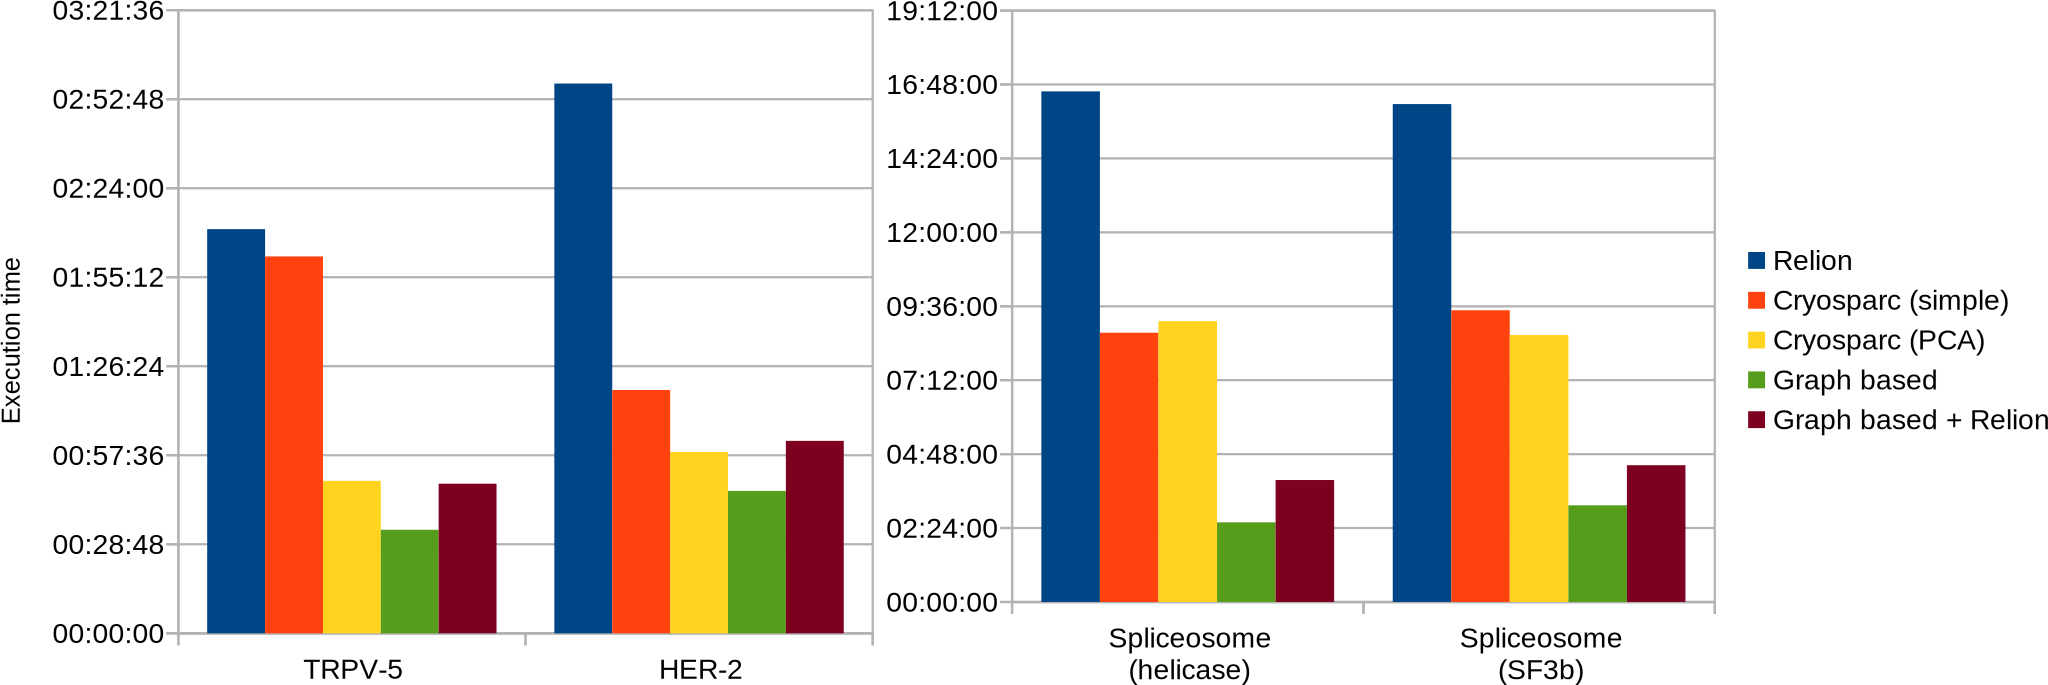
\includegraphics[width=\textwidth]{results/experiments/performance}
    \caption{Execution time comparison}
    \label{fig:5.2:performance}
\end{figure}

\end{document}
